\section{Spark::Sp\-Textured\-Grid\-Sg Class Reference}
\label{classSpark_1_1SpTexturedGridSg}\index{Spark::SpTexturedGridSg@{Spark::SpTexturedGridSg}}
{\tt \#include $<$Sp\-Textured\-Grid\-Sg.h$>$}

Inheritance diagram for Spark::Sp\-Textured\-Grid\-Sg:\begin{figure}[H]
\begin{center}
\leavevmode
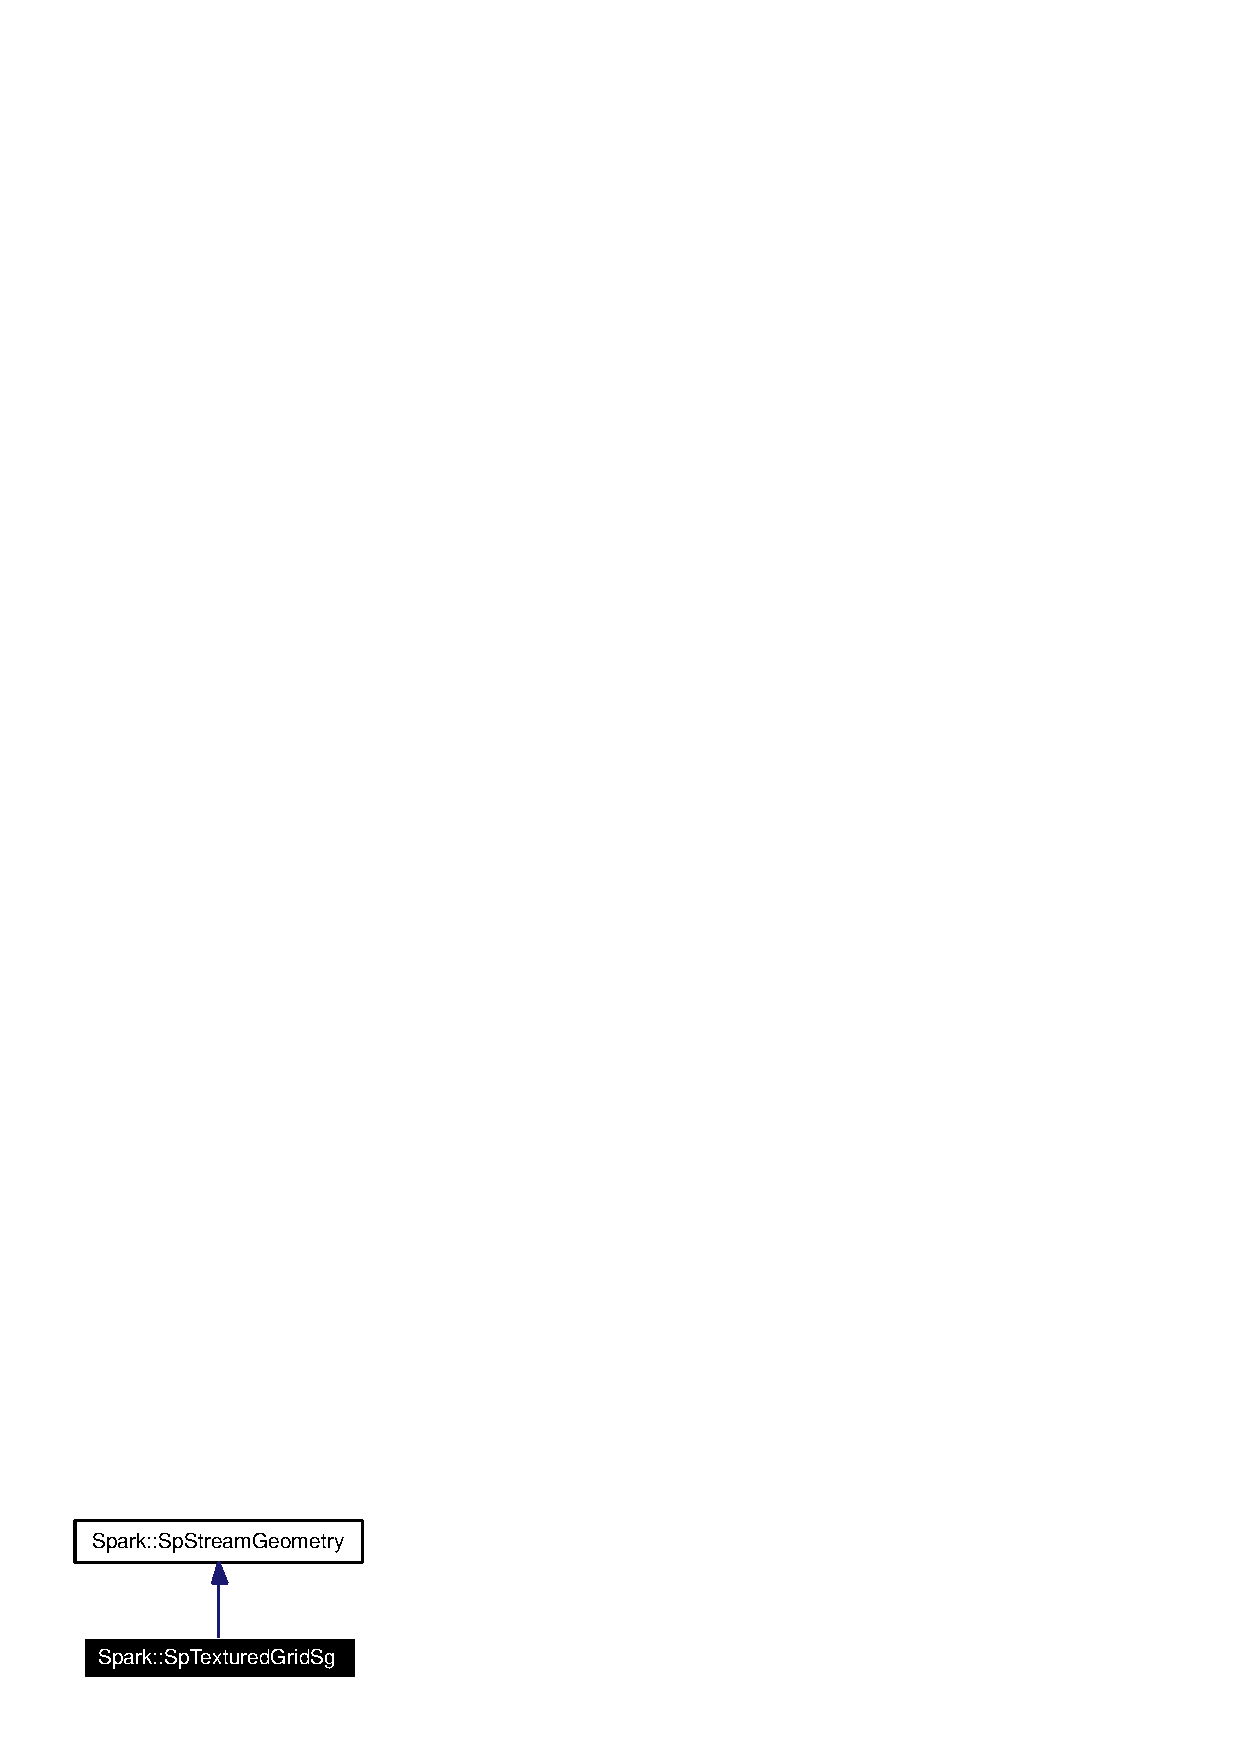
\includegraphics[width=87pt]{classSpark_1_1SpTexturedGridSg__inherit__graph}
\end{center}
\end{figure}
Collaboration diagram for Spark::Sp\-Textured\-Grid\-Sg:\begin{figure}[H]
\begin{center}
\leavevmode
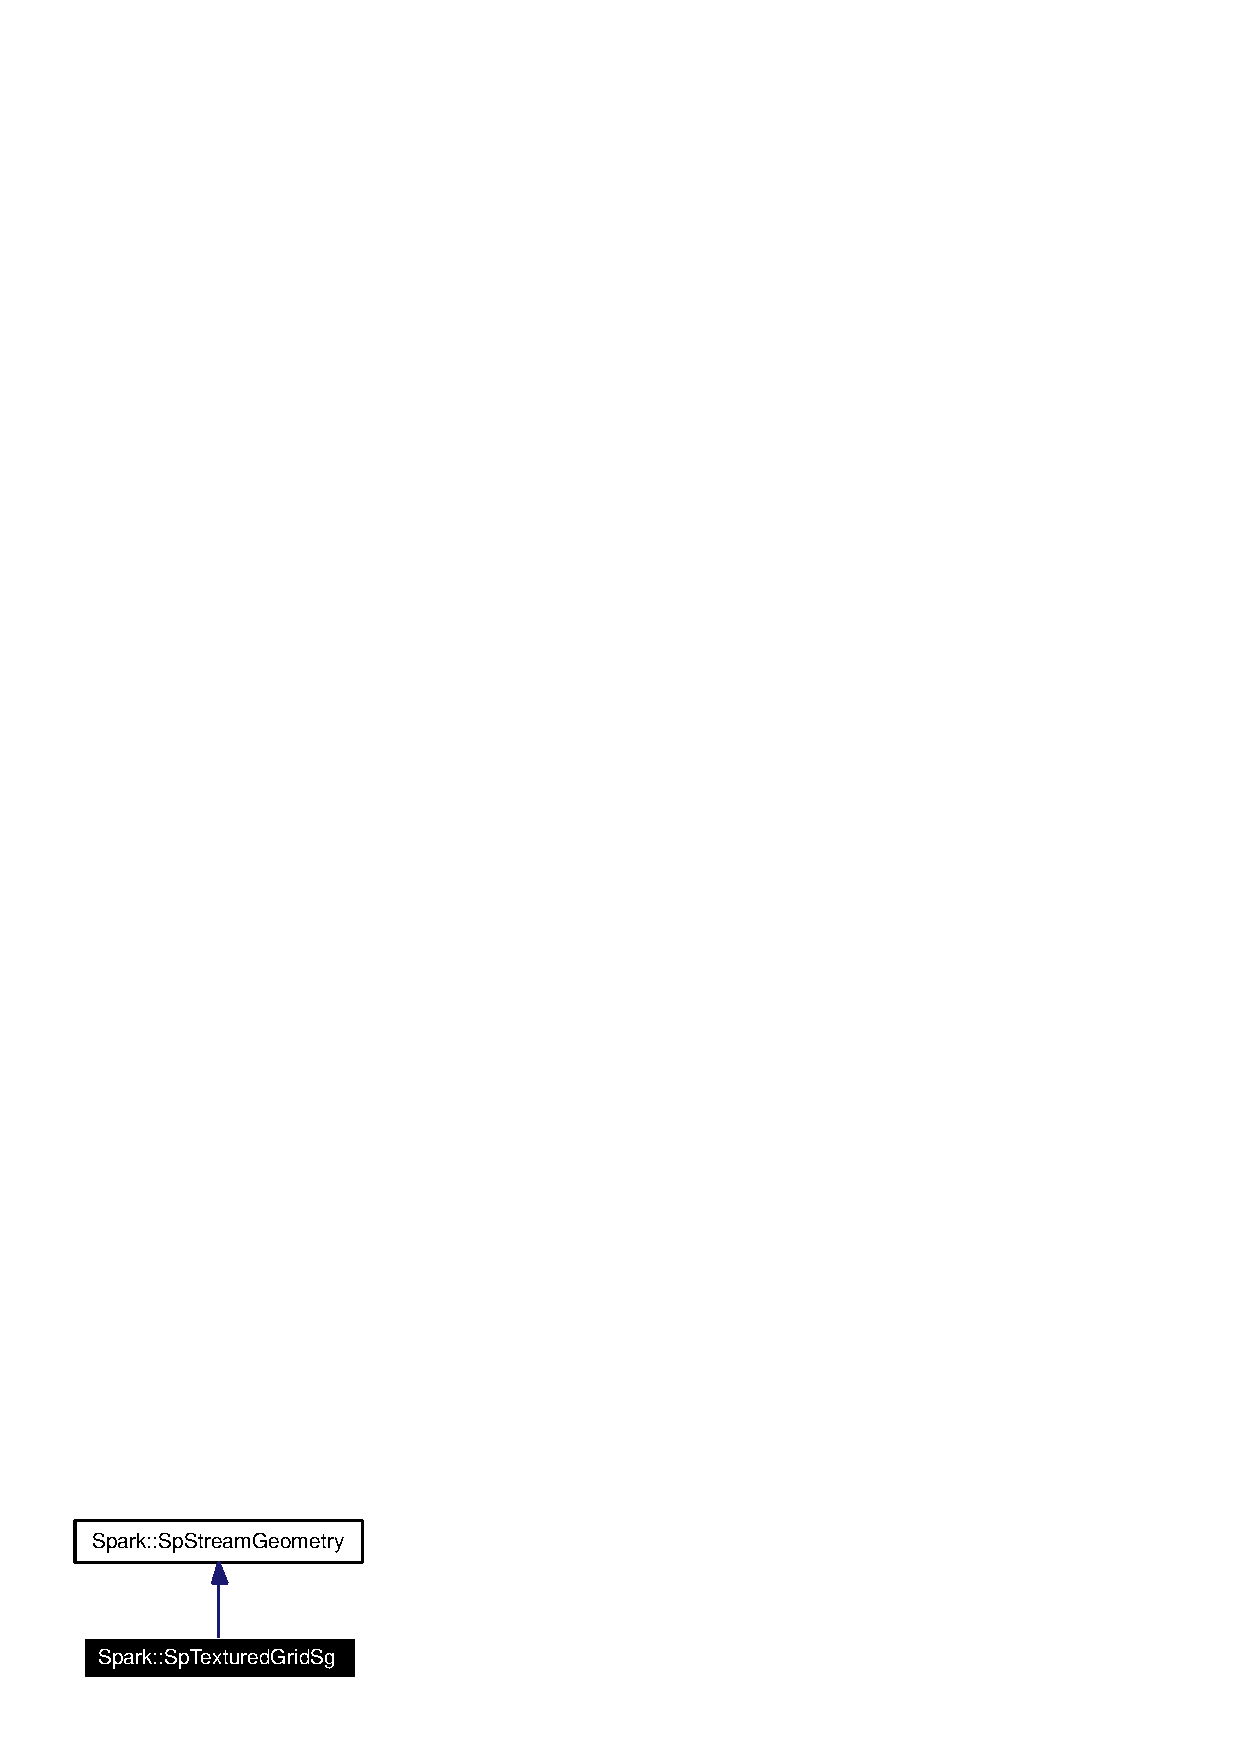
\includegraphics[width=87pt]{classSpark_1_1SpTexturedGridSg__coll__graph}
\end{center}
\end{figure}


\subsection{Detailed Description}
Multi-resolution grid-based stream geometry w/ texturing support. 

Definition at line 33 of file Sp\-Textured\-Grid\-Sg.h.\subsection*{Public Member Functions}
\begin{CompactItemize}
\item 
{\bf Sp\-Textured\-Grid\-Sg} (int i\-Rows=10, int i\-Cols=10, float f\-Min\-X=-1.0f, float f\-Min\-Y=-1.0f, float f\-Max\-X=1.0f, float f\-Max\-Y=1.0f, float f\-Z=0.0f, float f\-Min\-S=0.0f, float f\-Min\-T=0.0f, float f\-Max\-S=1.0f, float f\-Max\-T=1.0f)
\begin{CompactList}\small\item\em Construction:. \item\end{CompactList}\item 
virtual {\bf $\sim$Sp\-Textured\-Grid\-Sg} ()
\item 
virtual void {\bf render} ()
\begin{CompactList}\small\item\em Operations:. \item\end{CompactList}\item 
void {\bf set\-Resolution} (int i\-Rows, int i\-Cols)
\item 
void {\bf set\-Vertex\-Coord\-Rect} (float f\-Min\-X, float f\-Min\-Y, float f\-Max\-X, float f\-Max\-Y, float f\-Z=0.5f)
\item 
void {\bf set\-Tex\-Coord\-Rect} (float f\-Min\-S, float f\-Min\-T, float f\-Max\-S, float f\-Max\-T)
\end{CompactItemize}
\subsection*{Protected Attributes}
\begin{CompactItemize}
\item 
int {\bf m\_\-i\-Rows}
\begin{CompactList}\small\item\em Internal Data:. \item\end{CompactList}\item 
int {\bf m\_\-i\-Cols}
\item 
float {\bf m\_\-f\-Min\-X}
\item 
float {\bf m\_\-f\-Min\-Y}
\item 
float {\bf m\_\-f\-Max\-X}
\item 
float {\bf m\_\-f\-Max\-Y}
\item 
float {\bf m\_\-f\-Z}
\item 
float {\bf m\_\-f\-Min\-S}
\item 
float {\bf m\_\-f\-Max\-S}
\item 
float {\bf m\_\-f\-Min\-T}
\item 
float {\bf m\_\-f\-Max\-T}
\end{CompactItemize}


\subsection{Constructor \& Destructor Documentation}
\index{Spark::SpTexturedGridSg@{Spark::Sp\-Textured\-Grid\-Sg}!SpTexturedGridSg@{SpTexturedGridSg}}
\index{SpTexturedGridSg@{SpTexturedGridSg}!Spark::SpTexturedGridSg@{Spark::Sp\-Textured\-Grid\-Sg}}
\subsubsection{\setlength{\rightskip}{0pt plus 5cm}Spark::Sp\-Textured\-Grid\-Sg::Sp\-Textured\-Grid\-Sg (int {\em i\-Rows} = {\tt 10}, int {\em i\-Cols} = {\tt 10}, float {\em f\-Min\-X} = {\tt -1.0f}, float {\em f\-Min\-Y} = {\tt -1.0f}, float {\em f\-Max\-X} = {\tt 1.0f}, float {\em f\-Max\-Y} = {\tt 1.0f}, float {\em f\-Z} = {\tt 0.0f}, float {\em f\-Min\-S} = {\tt 0.0f}, float {\em f\-Min\-T} = {\tt 0.0f}, float {\em f\-Max\-S} = {\tt 1.0f}, float {\em f\-Max\-T} = {\tt 1.0f})\hspace{0.3cm}{\tt  [inline]}}\label{classSpark_1_1SpTexturedGridSg_a0}


Construction:. 

Definition at line 39 of file Sp\-Textured\-Grid\-Sg.h.

References m\_\-f\-Max\-S, m\_\-f\-Max\-T, m\_\-f\-Max\-X, m\_\-f\-Max\-Y, m\_\-f\-Min\-S, m\_\-f\-Min\-T, m\_\-f\-Min\-X, m\_\-f\-Min\-Y, m\_\-f\-Z, m\_\-i\-Cols, and m\_\-i\-Rows.\index{Spark::SpTexturedGridSg@{Spark::Sp\-Textured\-Grid\-Sg}!~SpTexturedGridSg@{$\sim$SpTexturedGridSg}}
\index{~SpTexturedGridSg@{$\sim$SpTexturedGridSg}!Spark::SpTexturedGridSg@{Spark::Sp\-Textured\-Grid\-Sg}}
\subsubsection{\setlength{\rightskip}{0pt plus 5cm}virtual Spark::Sp\-Textured\-Grid\-Sg::$\sim${\bf Sp\-Textured\-Grid\-Sg} ()\hspace{0.3cm}{\tt  [inline, virtual]}}\label{classSpark_1_1SpTexturedGridSg_a1}


Definition at line 55 of file Sp\-Textured\-Grid\-Sg.h.

\subsection{Member Function Documentation}
\index{Spark::SpTexturedGridSg@{Spark::Sp\-Textured\-Grid\-Sg}!render@{render}}
\index{render@{render}!Spark::SpTexturedGridSg@{Spark::Sp\-Textured\-Grid\-Sg}}
\subsubsection{\setlength{\rightskip}{0pt plus 5cm}virtual void Spark::Sp\-Textured\-Grid\-Sg::render ()\hspace{0.3cm}{\tt  [inline, virtual]}}\label{classSpark_1_1SpTexturedGridSg_a2}


Operations:. 



Implements {\bf Spark::Sp\-Stream\-Geometry} {\rm (p.\,\pageref{classSpark_1_1SpStreamGeometry_a0})}.

Definition at line 63 of file Sp\-Textured\-Grid\-Sg.h.

References m\_\-f\-Max\-S, m\_\-f\-Max\-T, m\_\-f\-Max\-X, m\_\-f\-Max\-Y, m\_\-f\-Min\-S, m\_\-f\-Min\-T, m\_\-f\-Min\-X, m\_\-f\-Min\-Y, m\_\-f\-Z, m\_\-i\-Cols, and m\_\-i\-Rows.

Referenced by Spark::Sp\-Vertex\-Noise\-Sb::send\-Output\-To\-Buffer().\index{Spark::SpTexturedGridSg@{Spark::Sp\-Textured\-Grid\-Sg}!setResolution@{setResolution}}
\index{setResolution@{setResolution}!Spark::SpTexturedGridSg@{Spark::Sp\-Textured\-Grid\-Sg}}
\subsubsection{\setlength{\rightskip}{0pt plus 5cm}void Spark::Sp\-Textured\-Grid\-Sg::set\-Resolution (int {\em i\-Rows}, int {\em i\-Cols})\hspace{0.3cm}{\tt  [inline]}}\label{classSpark_1_1SpTexturedGridSg_a3}


Definition at line 110 of file Sp\-Textured\-Grid\-Sg.h.

References m\_\-i\-Cols, and m\_\-i\-Rows.

Referenced by Spark::Sp\-Vertex\-Noise\-Sb::set\-Grid\-Resolution(), and Spark::Sp\-Vertex\-Noise\-Sb::Sp\-Vertex\-Noise\-Sb().\index{Spark::SpTexturedGridSg@{Spark::Sp\-Textured\-Grid\-Sg}!setTexCoordRect@{setTexCoordRect}}
\index{setTexCoordRect@{setTexCoordRect}!Spark::SpTexturedGridSg@{Spark::Sp\-Textured\-Grid\-Sg}}
\subsubsection{\setlength{\rightskip}{0pt plus 5cm}void Spark::Sp\-Textured\-Grid\-Sg::set\-Tex\-Coord\-Rect (float {\em f\-Min\-S}, float {\em f\-Min\-T}, float {\em f\-Max\-S}, float {\em f\-Max\-T})\hspace{0.3cm}{\tt  [inline]}}\label{classSpark_1_1SpTexturedGridSg_a5}


Definition at line 125 of file Sp\-Textured\-Grid\-Sg.h.

References m\_\-f\-Max\-S, m\_\-f\-Max\-T, m\_\-f\-Min\-S, and m\_\-f\-Min\-T.\index{Spark::SpTexturedGridSg@{Spark::Sp\-Textured\-Grid\-Sg}!setVertexCoordRect@{setVertexCoordRect}}
\index{setVertexCoordRect@{setVertexCoordRect}!Spark::SpTexturedGridSg@{Spark::Sp\-Textured\-Grid\-Sg}}
\subsubsection{\setlength{\rightskip}{0pt plus 5cm}void Spark::Sp\-Textured\-Grid\-Sg::set\-Vertex\-Coord\-Rect (float {\em f\-Min\-X}, float {\em f\-Min\-Y}, float {\em f\-Max\-X}, float {\em f\-Max\-Y}, float {\em f\-Z} = {\tt 0.5f})\hspace{0.3cm}{\tt  [inline]}}\label{classSpark_1_1SpTexturedGridSg_a4}


Definition at line 117 of file Sp\-Textured\-Grid\-Sg.h.

References m\_\-f\-Max\-X, m\_\-f\-Max\-Y, m\_\-f\-Min\-X, m\_\-f\-Min\-Y, and m\_\-f\-Z.

\subsection{Member Data Documentation}
\index{Spark::SpTexturedGridSg@{Spark::Sp\-Textured\-Grid\-Sg}!m_fMaxS@{m\_\-fMaxS}}
\index{m_fMaxS@{m\_\-fMaxS}!Spark::SpTexturedGridSg@{Spark::Sp\-Textured\-Grid\-Sg}}
\subsubsection{\setlength{\rightskip}{0pt plus 5cm}float {\bf Spark::Sp\-Textured\-Grid\-Sg::m\_\-f\-Max\-S}\hspace{0.3cm}{\tt  [protected]}}\label{classSpark_1_1SpTexturedGridSg_p8}


Definition at line 147 of file Sp\-Textured\-Grid\-Sg.h.

Referenced by render(), set\-Tex\-Coord\-Rect(), and Sp\-Textured\-Grid\-Sg().\index{Spark::SpTexturedGridSg@{Spark::Sp\-Textured\-Grid\-Sg}!m_fMaxT@{m\_\-fMaxT}}
\index{m_fMaxT@{m\_\-fMaxT}!Spark::SpTexturedGridSg@{Spark::Sp\-Textured\-Grid\-Sg}}
\subsubsection{\setlength{\rightskip}{0pt plus 5cm}float {\bf Spark::Sp\-Textured\-Grid\-Sg::m\_\-f\-Max\-T}\hspace{0.3cm}{\tt  [protected]}}\label{classSpark_1_1SpTexturedGridSg_p10}


Definition at line 149 of file Sp\-Textured\-Grid\-Sg.h.

Referenced by render(), set\-Tex\-Coord\-Rect(), and Sp\-Textured\-Grid\-Sg().\index{Spark::SpTexturedGridSg@{Spark::Sp\-Textured\-Grid\-Sg}!m_fMaxX@{m\_\-fMaxX}}
\index{m_fMaxX@{m\_\-fMaxX}!Spark::SpTexturedGridSg@{Spark::Sp\-Textured\-Grid\-Sg}}
\subsubsection{\setlength{\rightskip}{0pt plus 5cm}float {\bf Spark::Sp\-Textured\-Grid\-Sg::m\_\-f\-Max\-X}\hspace{0.3cm}{\tt  [protected]}}\label{classSpark_1_1SpTexturedGridSg_p4}


Definition at line 141 of file Sp\-Textured\-Grid\-Sg.h.

Referenced by render(), set\-Vertex\-Coord\-Rect(), and Sp\-Textured\-Grid\-Sg().\index{Spark::SpTexturedGridSg@{Spark::Sp\-Textured\-Grid\-Sg}!m_fMaxY@{m\_\-fMaxY}}
\index{m_fMaxY@{m\_\-fMaxY}!Spark::SpTexturedGridSg@{Spark::Sp\-Textured\-Grid\-Sg}}
\subsubsection{\setlength{\rightskip}{0pt plus 5cm}float {\bf Spark::Sp\-Textured\-Grid\-Sg::m\_\-f\-Max\-Y}\hspace{0.3cm}{\tt  [protected]}}\label{classSpark_1_1SpTexturedGridSg_p5}


Definition at line 142 of file Sp\-Textured\-Grid\-Sg.h.

Referenced by render(), set\-Vertex\-Coord\-Rect(), and Sp\-Textured\-Grid\-Sg().\index{Spark::SpTexturedGridSg@{Spark::Sp\-Textured\-Grid\-Sg}!m_fMinS@{m\_\-fMinS}}
\index{m_fMinS@{m\_\-fMinS}!Spark::SpTexturedGridSg@{Spark::Sp\-Textured\-Grid\-Sg}}
\subsubsection{\setlength{\rightskip}{0pt plus 5cm}float {\bf Spark::Sp\-Textured\-Grid\-Sg::m\_\-f\-Min\-S}\hspace{0.3cm}{\tt  [protected]}}\label{classSpark_1_1SpTexturedGridSg_p7}


Definition at line 146 of file Sp\-Textured\-Grid\-Sg.h.

Referenced by render(), set\-Tex\-Coord\-Rect(), and Sp\-Textured\-Grid\-Sg().\index{Spark::SpTexturedGridSg@{Spark::Sp\-Textured\-Grid\-Sg}!m_fMinT@{m\_\-fMinT}}
\index{m_fMinT@{m\_\-fMinT}!Spark::SpTexturedGridSg@{Spark::Sp\-Textured\-Grid\-Sg}}
\subsubsection{\setlength{\rightskip}{0pt plus 5cm}float {\bf Spark::Sp\-Textured\-Grid\-Sg::m\_\-f\-Min\-T}\hspace{0.3cm}{\tt  [protected]}}\label{classSpark_1_1SpTexturedGridSg_p9}


Definition at line 148 of file Sp\-Textured\-Grid\-Sg.h.

Referenced by render(), set\-Tex\-Coord\-Rect(), and Sp\-Textured\-Grid\-Sg().\index{Spark::SpTexturedGridSg@{Spark::Sp\-Textured\-Grid\-Sg}!m_fMinX@{m\_\-fMinX}}
\index{m_fMinX@{m\_\-fMinX}!Spark::SpTexturedGridSg@{Spark::Sp\-Textured\-Grid\-Sg}}
\subsubsection{\setlength{\rightskip}{0pt plus 5cm}float {\bf Spark::Sp\-Textured\-Grid\-Sg::m\_\-f\-Min\-X}\hspace{0.3cm}{\tt  [protected]}}\label{classSpark_1_1SpTexturedGridSg_p2}


Definition at line 139 of file Sp\-Textured\-Grid\-Sg.h.

Referenced by render(), set\-Vertex\-Coord\-Rect(), and Sp\-Textured\-Grid\-Sg().\index{Spark::SpTexturedGridSg@{Spark::Sp\-Textured\-Grid\-Sg}!m_fMinY@{m\_\-fMinY}}
\index{m_fMinY@{m\_\-fMinY}!Spark::SpTexturedGridSg@{Spark::Sp\-Textured\-Grid\-Sg}}
\subsubsection{\setlength{\rightskip}{0pt plus 5cm}float {\bf Spark::Sp\-Textured\-Grid\-Sg::m\_\-f\-Min\-Y}\hspace{0.3cm}{\tt  [protected]}}\label{classSpark_1_1SpTexturedGridSg_p3}


Definition at line 140 of file Sp\-Textured\-Grid\-Sg.h.

Referenced by render(), set\-Vertex\-Coord\-Rect(), and Sp\-Textured\-Grid\-Sg().\index{Spark::SpTexturedGridSg@{Spark::Sp\-Textured\-Grid\-Sg}!m_fZ@{m\_\-fZ}}
\index{m_fZ@{m\_\-fZ}!Spark::SpTexturedGridSg@{Spark::Sp\-Textured\-Grid\-Sg}}
\subsubsection{\setlength{\rightskip}{0pt plus 5cm}float {\bf Spark::Sp\-Textured\-Grid\-Sg::m\_\-f\-Z}\hspace{0.3cm}{\tt  [protected]}}\label{classSpark_1_1SpTexturedGridSg_p6}


Definition at line 144 of file Sp\-Textured\-Grid\-Sg.h.

Referenced by render(), set\-Vertex\-Coord\-Rect(), and Sp\-Textured\-Grid\-Sg().\index{Spark::SpTexturedGridSg@{Spark::Sp\-Textured\-Grid\-Sg}!m_iCols@{m\_\-iCols}}
\index{m_iCols@{m\_\-iCols}!Spark::SpTexturedGridSg@{Spark::Sp\-Textured\-Grid\-Sg}}
\subsubsection{\setlength{\rightskip}{0pt plus 5cm}int {\bf Spark::Sp\-Textured\-Grid\-Sg::m\_\-i\-Cols}\hspace{0.3cm}{\tt  [protected]}}\label{classSpark_1_1SpTexturedGridSg_p1}


Definition at line 137 of file Sp\-Textured\-Grid\-Sg.h.

Referenced by render(), set\-Resolution(), and Sp\-Textured\-Grid\-Sg().\index{Spark::SpTexturedGridSg@{Spark::Sp\-Textured\-Grid\-Sg}!m_iRows@{m\_\-iRows}}
\index{m_iRows@{m\_\-iRows}!Spark::SpTexturedGridSg@{Spark::Sp\-Textured\-Grid\-Sg}}
\subsubsection{\setlength{\rightskip}{0pt plus 5cm}int {\bf Spark::Sp\-Textured\-Grid\-Sg::m\_\-i\-Rows}\hspace{0.3cm}{\tt  [protected]}}\label{classSpark_1_1SpTexturedGridSg_p0}


Internal Data:. 

Definition at line 136 of file Sp\-Textured\-Grid\-Sg.h.

Referenced by render(), set\-Resolution(), and Sp\-Textured\-Grid\-Sg().

The documentation for this class was generated from the following file:\begin{CompactItemize}
\item 
{\bf Sp\-Textured\-Grid\-Sg.h}\end{CompactItemize}
